\documentclass{article}
\usepackage[utf8]{inputenc}
\usepackage{amsmath}
\usepackage{amsfonts}
\usepackage{amssymb}
\usepackage{graphicx}
\usepackage{geometry}
\usepackage{xcolor}
\usepackage{gensymb}
\usepackage{hyperref}
\usepackage{gensymb}
\usepackage{listings}

\newcommand{\inv}{^{-1}}   
\newcommand{\Z}{\mathbb Z}
\newcommand{\R}{\mathbb R}
\newcommand{\Q}{\mathbb Q}
\newcommand{\C}{\mathbb C}
\newcommand{\N}{\mathbb N}

\begin{document}

\medskip\noindent\textbf{1.} 

    Here's my 12V power supply:
    \begin{center} 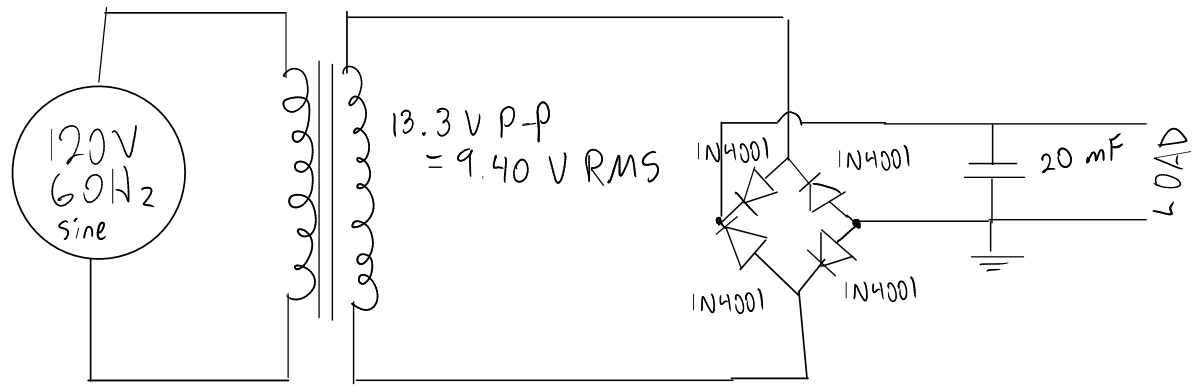
\includegraphics[scale=.3]{power_supply.png} \end{center}

    I solved for the capacitance using $V_{\text{ripple}} = \frac{I_{\text{out}}}{fC},$ and arrived at $C = \frac{1}{48} \approx 20$mF.

\medskip\noindent\textbf{2.} 

    Gain = $\frac{R_1 + R_2}{R_1} = \frac{64}{8} = 8.$

    The figure below shows $\text{V}_{\text{in}}$ in red and $\text{V}_{\text{out}}$ in blue.
    \begin{center}
        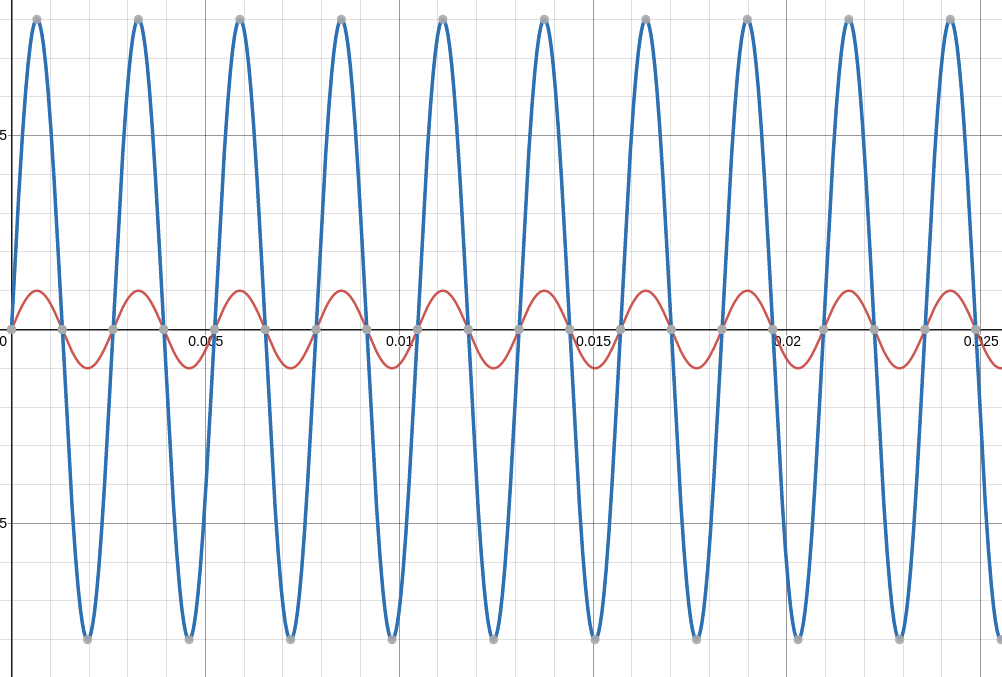
\includegraphics[scale=.3]{2.png}
    \end{center}

\newpage\noindent\textbf{3.}

\medskip\noindent\textbf{4.}

    Obvious answer is -10Vin.

    Real answer comes from thinking about currents.

\medskip\noindent\textbf{5.} Because it doesn't pull any current from the input 

\medskip\noindent\textbf{6.}

\newpage\noindent\textbf{7.} 
    
\medskip\noindent\textbf{8.}

\newpage\noindent\textbf{9.}

\medskip\noindent\textbf{10.}

\end{document}
